\ylDisplay{Plokid} % Ülesande nimi
{Koit Timpmann} % Autor
{lõppvoor} % Voor
{2019} % Aasta
{P 3} % Ülesande nr.
{2} % Raskustase
{
% Teema: Mehaanika
\ifStatement
Süsteem koosneb ühest liikuvast ja ühest liikumatust plokist ning kahest koormisest massidega $m_1 = 150$ $g$ ja $m_2 = 100$ g (vt joonist). Koormisi hoitakse paigal ning lastakse siis lahti. Kui suur on koormise $m_1$ kiirus hetkel, kui see on läbinud vahemaa $s = 0,5$ m. Plokkide massi ja hõõrdumist süsteemis ei ole tarvis arvestada.
\begin{center}
	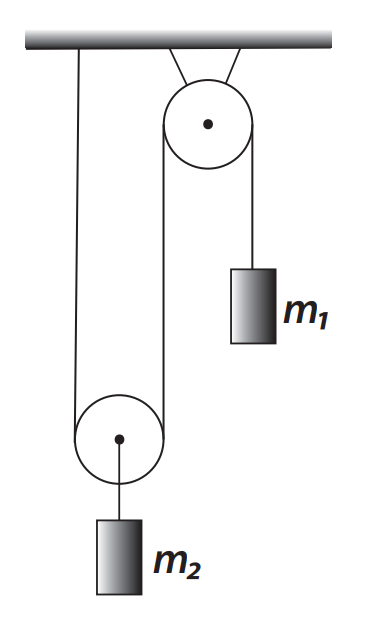
\includegraphics[width=0.5\linewidth]{2019-v3p-03-yl.PNG}
\end{center}
\fi

\ifHint
Plokkide liikumisel kõrguste vahest tingitud potentsiaalse energia muutus muundub plokkide kineetiliseks energiaks. Plokkide kineetiliste energiate muutuste summa peab olema võrdne potentsiaalsete energiate muutumise summaga.
\fi

\ifSolution
Lähtume energia jäävuse seadusest. Süsteemi kineetiline energia hetkel, kui koormis $m_1$ on läbinud vahemaa $s$ võrdub süsteemi potentsiaalse energia muuduga. Kuna koormis $m_2$ ripub liikuva ploki otsas, siis on selle koormise poolt läbitud tee antud ajahetkeks kaks korda lühem kui koormise $m_1$ poolt läbitud tee ning selle kiirus samuti kaks korda väiksem koormise $m_1$ kiirusest.
Seega: 
\begin{center}
$\frac{m_1 v^2}{2} + \frac{m_2(0,5v)^2}{2} = m_1ga - m_2g\frac{s}{2}$,
\end{center}
millest
\begin{center}
$v = 2\sqrt{\frac{(2m_1 - m_2)gs}{4m_1 + m_2}} \approx 2,37$ $m/s$.
\end{center}
\fi
}